\subsection{Main controller}

På figur \ref{fig:ibd_maincontroller} vises et ibd over main controlleren. Diagrammet viser de interne forbindelser i main controlleren. Sammenlignes main controller og drone ibd er den eneste forskel at der på nedenstående ibd kan ses hvordan main controlleren forsynes.  

\begin{figure}[H]
\centering
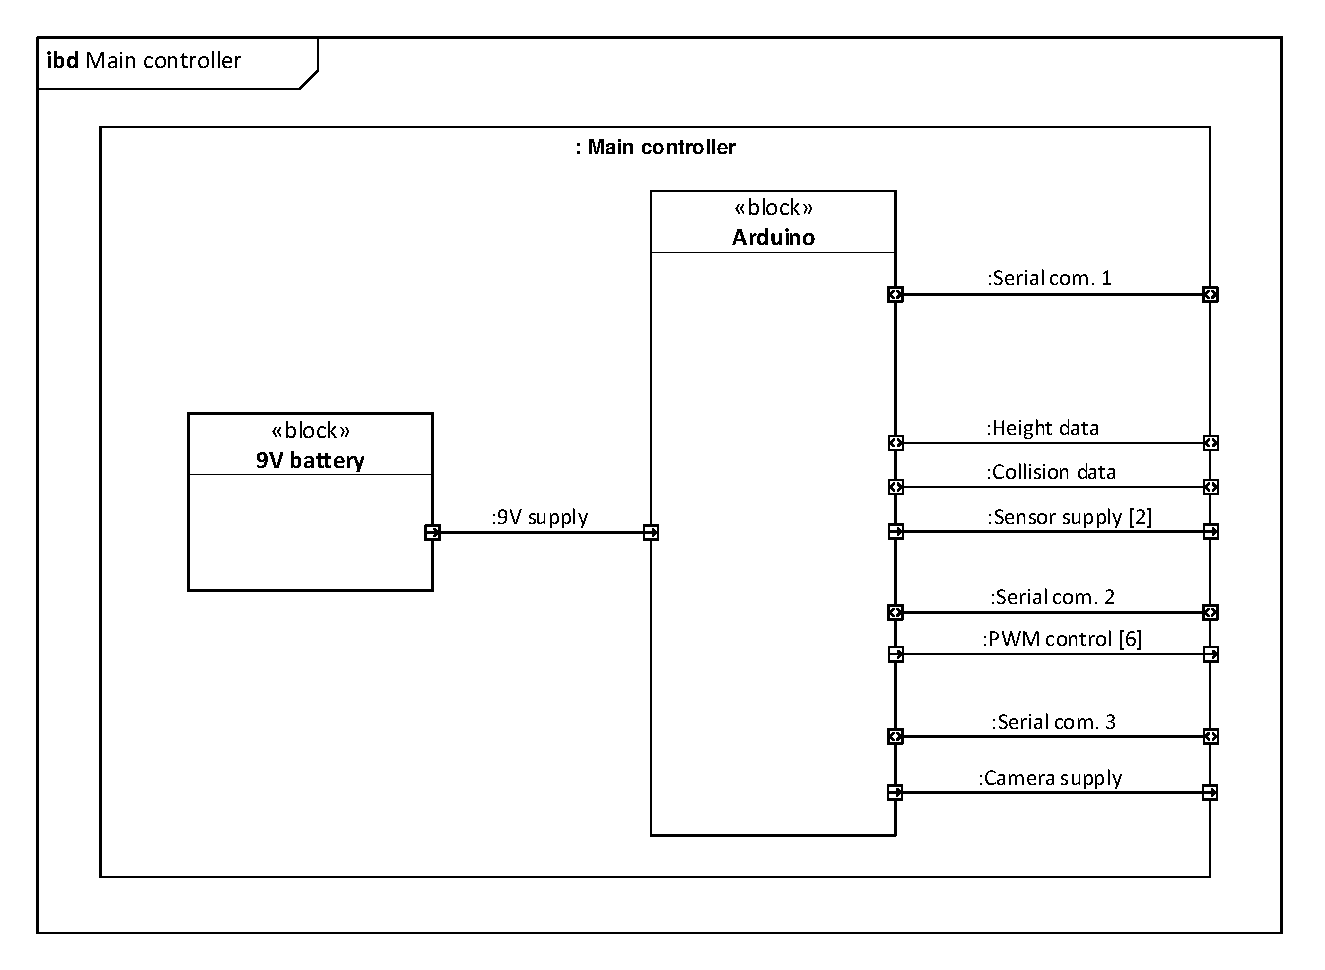
\includegraphics[width=1\textwidth]{Billeder/IBD/ibd3_maincontroller.pdf}
\vspace{-1cm}
\caption{Ibd - Main controller}
\label{fig:ibd_maincontroller}
\end{figure}

\begin{table}[H]
	\centering
		\begin{tabular}{|p{2.6 cm}|p{4.9 cm}|p{2.5 cm}|p{2.5 cm}|}  
		\hline
			\textbf{Signal navn} 	& \textbf{Signal beskrivelse}		& \textbf{Out} 				& \textbf{In}     \\ \hline
			9V supply & Forsyning til Arduino. & 9V battery. & Arduino. 		    \\ \hline
			Serial com. 1		& RX / TX signal. Styrer 3G modul. 	& Main controller. 	& 3G/GPS    \\ \hline
			Height data		& Trigger \& echo signal der indikerer afstanden. 	& Main controller.	& Distance sensors.	\\ \hline
			Kollision data	& Trigger \& echo signal der indikerer afstanden. 	& Main controller.	& Distance sensors.  \\ \hline
			Sensor supply [2]	& 5V DC forsyning.	& Main controller. & Distance sensors.	\\ \hline
			Serial com. 2		& RX / TX signal. Aflæser data fra kompas & Main controller.				& Flight control board. 	\\ \hline 
			PWM control [6]		& 50 Hz 6 kanals signal. Duty cycle 5-10\%. Periode på 20ms.	& Main controller.				& Flight control board.	\\ \hline
			Serial com. 3		& RX / TX signal. Styrer kamera	& Main controller.	& Camera.	\\ \hline
			Cam supply			& 5V DC forsyning. 	& Main controller.	& Camera.	\\ \hline 
		\end{tabular}
	\caption{Forbindelser til: Ibd - Main controller}
	\label{tab:IBDMaincontroller}
\end{table}

